\section{eo\-Additive\-Binary\-Epsilon\-Indicator$<$ EOFitness $>$ Class Template Reference}
\label{classeoAdditiveBinaryEpsilonIndicator}\index{eoAdditiveBinaryEpsilonIndicator@{eoAdditiveBinaryEpsilonIndicator}}
Functor Additive binary epsilon indicator for {\bf eo\-Pareto\-Fitness}.  


{\tt \#include $<$eo\-Binary\-Quality\-Indicator.h$>$}

Inheritance diagram for eo\-Additive\-Binary\-Epsilon\-Indicator$<$ EOFitness $>$::\begin{figure}[H]
\begin{center}
\leavevmode
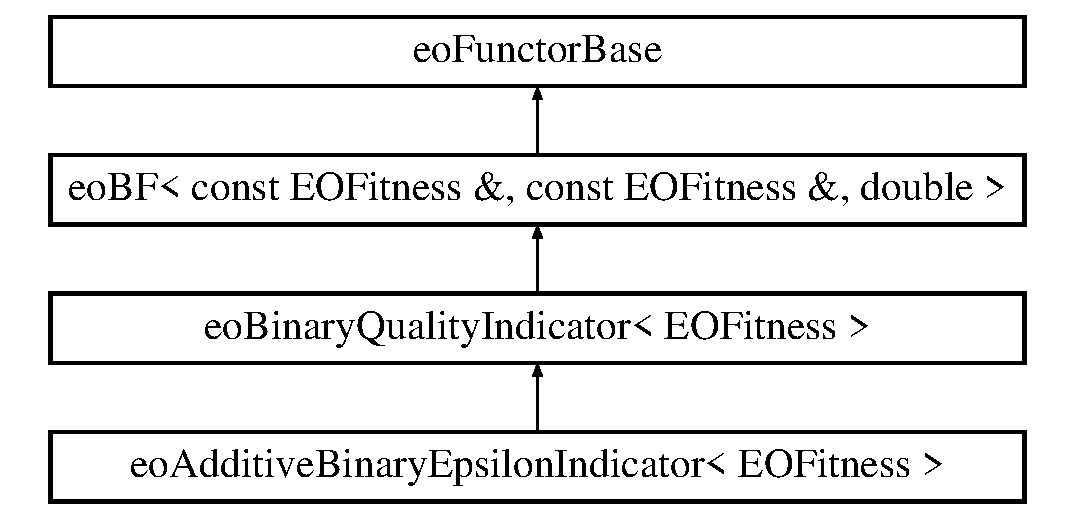
\includegraphics[height=4cm]{classeoAdditiveBinaryEpsilonIndicator}
\end{center}
\end{figure}
\subsection*{Public Member Functions}
\begin{CompactItemize}
\item 
{\bf eo\-Additive\-Binary\-Epsilon\-Indicator} ()\label{classeoAdditiveBinaryEpsilonIndicator_c76501f3d05bc3c1e9ccef6f9c465cb9}

\begin{CompactList}\small\item\em constructor \item\end{CompactList}\item 
double {\bf operator()} (const EOFitness \&\_\-fitness\_\-eo1, const EOFitness \&\_\-fitness\_\-eo2)
\begin{CompactList}\small\item\em computation of the maximum epsilon value by which individual \_\-eo1 must be decreased in all objectives such that individual \_\-eo2 is weakly dominated (do not forget to set the bounds before the call of this function) \item\end{CompactList}\end{CompactItemize}
\subsection*{Private Types}
\begin{CompactItemize}
\item 
typedef EOFitness::fitness\_\-traits {\bf traits}\label{classeoAdditiveBinaryEpsilonIndicator_c6d4c79183683a05183a31fcb7f533f1}

\begin{CompactList}\small\item\em fitness traits \item\end{CompactList}\end{CompactItemize}
\subsection*{Private Member Functions}
\begin{CompactItemize}
\item 
double {\bf epsilon\-Value} (const EOFitness \&\_\-fitness\_\-eo1, const EOFitness \&\_\-fitness\_\-eo2, const unsigned \_\-i\-Obj)
\begin{CompactList}\small\item\em computation of the epsilon value by which individual \_\-eo1 must be decreased in the objective \_\-i\-Obj such that individual \_\-eo2 is weakly dominated \item\end{CompactList}\end{CompactItemize}


\subsection{Detailed Description}
\subsubsection*{template$<$class EOFitness$>$ class eo\-Additive\-Binary\-Epsilon\-Indicator$<$ EOFitness $>$}

Functor Additive binary epsilon indicator for {\bf eo\-Pareto\-Fitness}. 



Definition at line 126 of file eo\-Binary\-Quality\-Indicator.h.

\subsection{Member Function Documentation}
\index{eoAdditiveBinaryEpsilonIndicator@{eo\-Additive\-Binary\-Epsilon\-Indicator}!operator()@{operator()}}
\index{operator()@{operator()}!eoAdditiveBinaryEpsilonIndicator@{eo\-Additive\-Binary\-Epsilon\-Indicator}}
\subsubsection{\setlength{\rightskip}{0pt plus 5cm}template$<$class EOFitness$>$ double {\bf eo\-Additive\-Binary\-Epsilon\-Indicator}$<$ EOFitness $>$::operator() (const EOFitness \& {\em \_\-fitness\_\-eo1}, const EOFitness \& {\em \_\-fitness\_\-eo2})\hspace{0.3cm}{\tt  [inline, virtual]}}\label{classeoAdditiveBinaryEpsilonIndicator_5fd885a2a555e26706174a44ef636f4d}


computation of the maximum epsilon value by which individual \_\-eo1 must be decreased in all objectives such that individual \_\-eo2 is weakly dominated (do not forget to set the bounds before the call of this function) 

\begin{Desc}
\item[Parameters:]
\begin{description}
\item[{\em EOFitness}]\& \_\-fitness\_\-eo1 the fitness of the first individual \item[{\em EOFitness}]\& \_\-fitness\_\-eo2 the fitness of the second individual \end{description}
\end{Desc}


Implements {\bf eo\-BF$<$ const EOFitness \&, const EOFitness \&, double $>$}.

Definition at line 149 of file eo\-Binary\-Quality\-Indicator.h.

References eo\-Additive\-Binary\-Epsilon\-Indicator$<$ EOFitness $>$::epsilon\-Value().\index{eoAdditiveBinaryEpsilonIndicator@{eo\-Additive\-Binary\-Epsilon\-Indicator}!epsilonValue@{epsilonValue}}
\index{epsilonValue@{epsilonValue}!eoAdditiveBinaryEpsilonIndicator@{eo\-Additive\-Binary\-Epsilon\-Indicator}}
\subsubsection{\setlength{\rightskip}{0pt plus 5cm}template$<$class EOFitness$>$ double {\bf eo\-Additive\-Binary\-Epsilon\-Indicator}$<$ EOFitness $>$::epsilon\-Value (const EOFitness \& {\em \_\-fitness\_\-eo1}, const EOFitness \& {\em \_\-fitness\_\-eo2}, const unsigned {\em \_\-i\-Obj})\hspace{0.3cm}{\tt  [inline, private]}}\label{classeoAdditiveBinaryEpsilonIndicator_8f35162769a1b23ada83e5fb21cc74e7}


computation of the epsilon value by which individual \_\-eo1 must be decreased in the objective \_\-i\-Obj such that individual \_\-eo2 is weakly dominated 

\begin{Desc}
\item[Parameters:]
\begin{description}
\item[{\em EOFitness}]\& \_\-fitness\_\-eo1 the fitness of the first individual \item[{\em EOFitness}]\& \_\-fitness\_\-eo2 the fitness of the second individual \item[{\em unsigned}]\_\-i\-Obj the index of the objective \end{description}
\end{Desc}


Definition at line 181 of file eo\-Binary\-Quality\-Indicator.h.

Referenced by eo\-Additive\-Binary\-Epsilon\-Indicator$<$ EOFitness $>$::operator()().

The documentation for this class was generated from the following file:\begin{CompactItemize}
\item 
eo\-Binary\-Quality\-Indicator.h\end{CompactItemize}
